%\begin{tcolorbox}[breakable,colback=black!5!white,colframe=red!80!black,width=\textwidth]
\chapter{The Large Hadron Collider and the CMS experiment}
%\end{tcolorbox}
\label{chap:LHC_CMS}

\section{The Large Hadron Collider}
The Large Hadron Collider (LHC) is a 27 km ring structure designed for the acceleartion and collision of protons and heavy ions. It is situated approximatively 100 m underground, between France and Switzerland, in the Geneva area, and it is the most important of the CERN (Conseil europ\'een pour la recherche nucl\'eaire) facilities. It has been designed to fit the pre-existing underground tunnel of the LEP collider [ref. 24 Jacopo], built to accelerate electrons and positrons until the year 2000, in order to reduce the cost of the project, definetively approved in 1996.\\
Moving from an electron-positron collider to an hadron collider allowed to reach higher energies in the center-of-mass frame, since the syncrotron radiation loss is inversely proportional to the fourth power of the mass of the particle involved: hence, it is reduced by a factor $m_p/m_e \sim 10^3$. Furthermore, at a proton-proton collider it is possible to collect higher luminosities (and hence more statistics) with regards to, for example, a proton-antiproton collider, like Tevatron at Fermilab, in the USA.\\
In the LHC two identical beam pipes rings are designed to let protons circulate in opposite directions, in ultrahigh vacuum conditions ($10^{-13}$ atm) in order to avoid collisions with gas molecules. 

LHC \`e dotato di due anelli identici, entro cui i fasci di particelle corrono in direzioni opposte in tubi a vuoto. La geometria di LHC si basa su quella precedente di LEP: l'acceleratore \`e diviso in 8 strutture ad arco per la curvatura delle traiettorie e in segmenti lunghi 520 m utili per l'iniezione e per strumenti di controllo del sistema. I fasci di protoni collidono in 4 punti di interazione, nei quali sono installati i quattro principali rivelatori: ALICE, ATLAS, CMS, LHCb.

\begin{figure}[!htb]
  \centering
    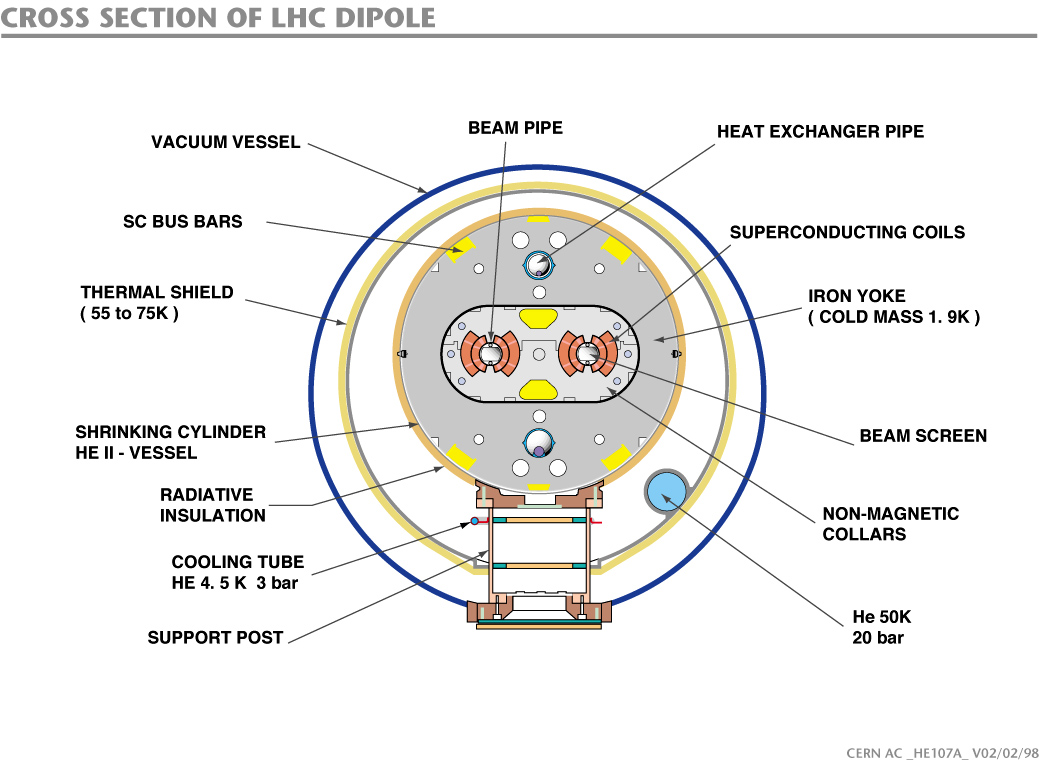
\includegraphics[width=.75\textwidth]{figures/LHC-magnets.jpg}
  \caption{Sezione della struttura ad arco per la curvatura delle traiettorie dei protoni.}
  \label{fig:LHC_dipole}
\end{figure}

\noindent Il ridotto diametro interno del tunnel, di circa 4 m, ha comportato delle limitazioni nella costruzione dei magneti superconduttori, costringendo ad accoppiare magneticamente i due fasci. In figura \ref{fig:dipolo} \`e mostrata una sezione delle strutture ad arco. Attorno ai tubi di fascio sono disposti due magneti dipolari a superconduttore, essi generano due campi magnetici verticali paralleli e discordi e sono preposti alla curvatura delle traiettorie. Oltre a questi, si trovano magneti quadrupolari, utili per la focalizzazione dei fasci, e altri piccoli magneti con sei o otto poli per piccole correzioni sulla dimensione dei fasci e sulla loro posizione. Tutti i magneti e le cavit\`a acceleratrici sono costruite in metalli (titanio e niobio) superconduttori, che vengono raffreddati a $-271.3^{\circ}$C (1.9K) con sistemi ad elio liquido. In LHC ci sono un totale di 1232 magneti dipolari e 392 quadrupolari, capaci di creare un campo magnetico massimo di 8.33 T.

\begin{figure}[!htb]
  \centering
    %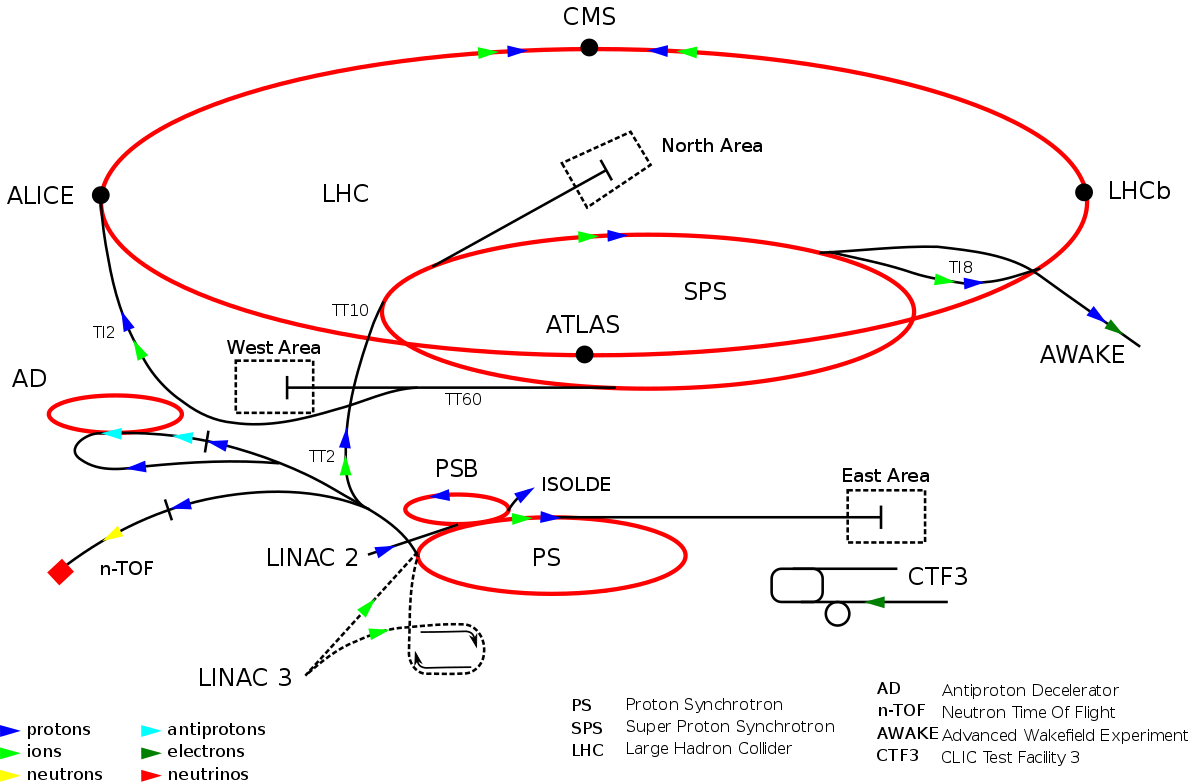
\includegraphics[width=.75\textwidth]{figures/Cern-accelerator-complex.png}\\
    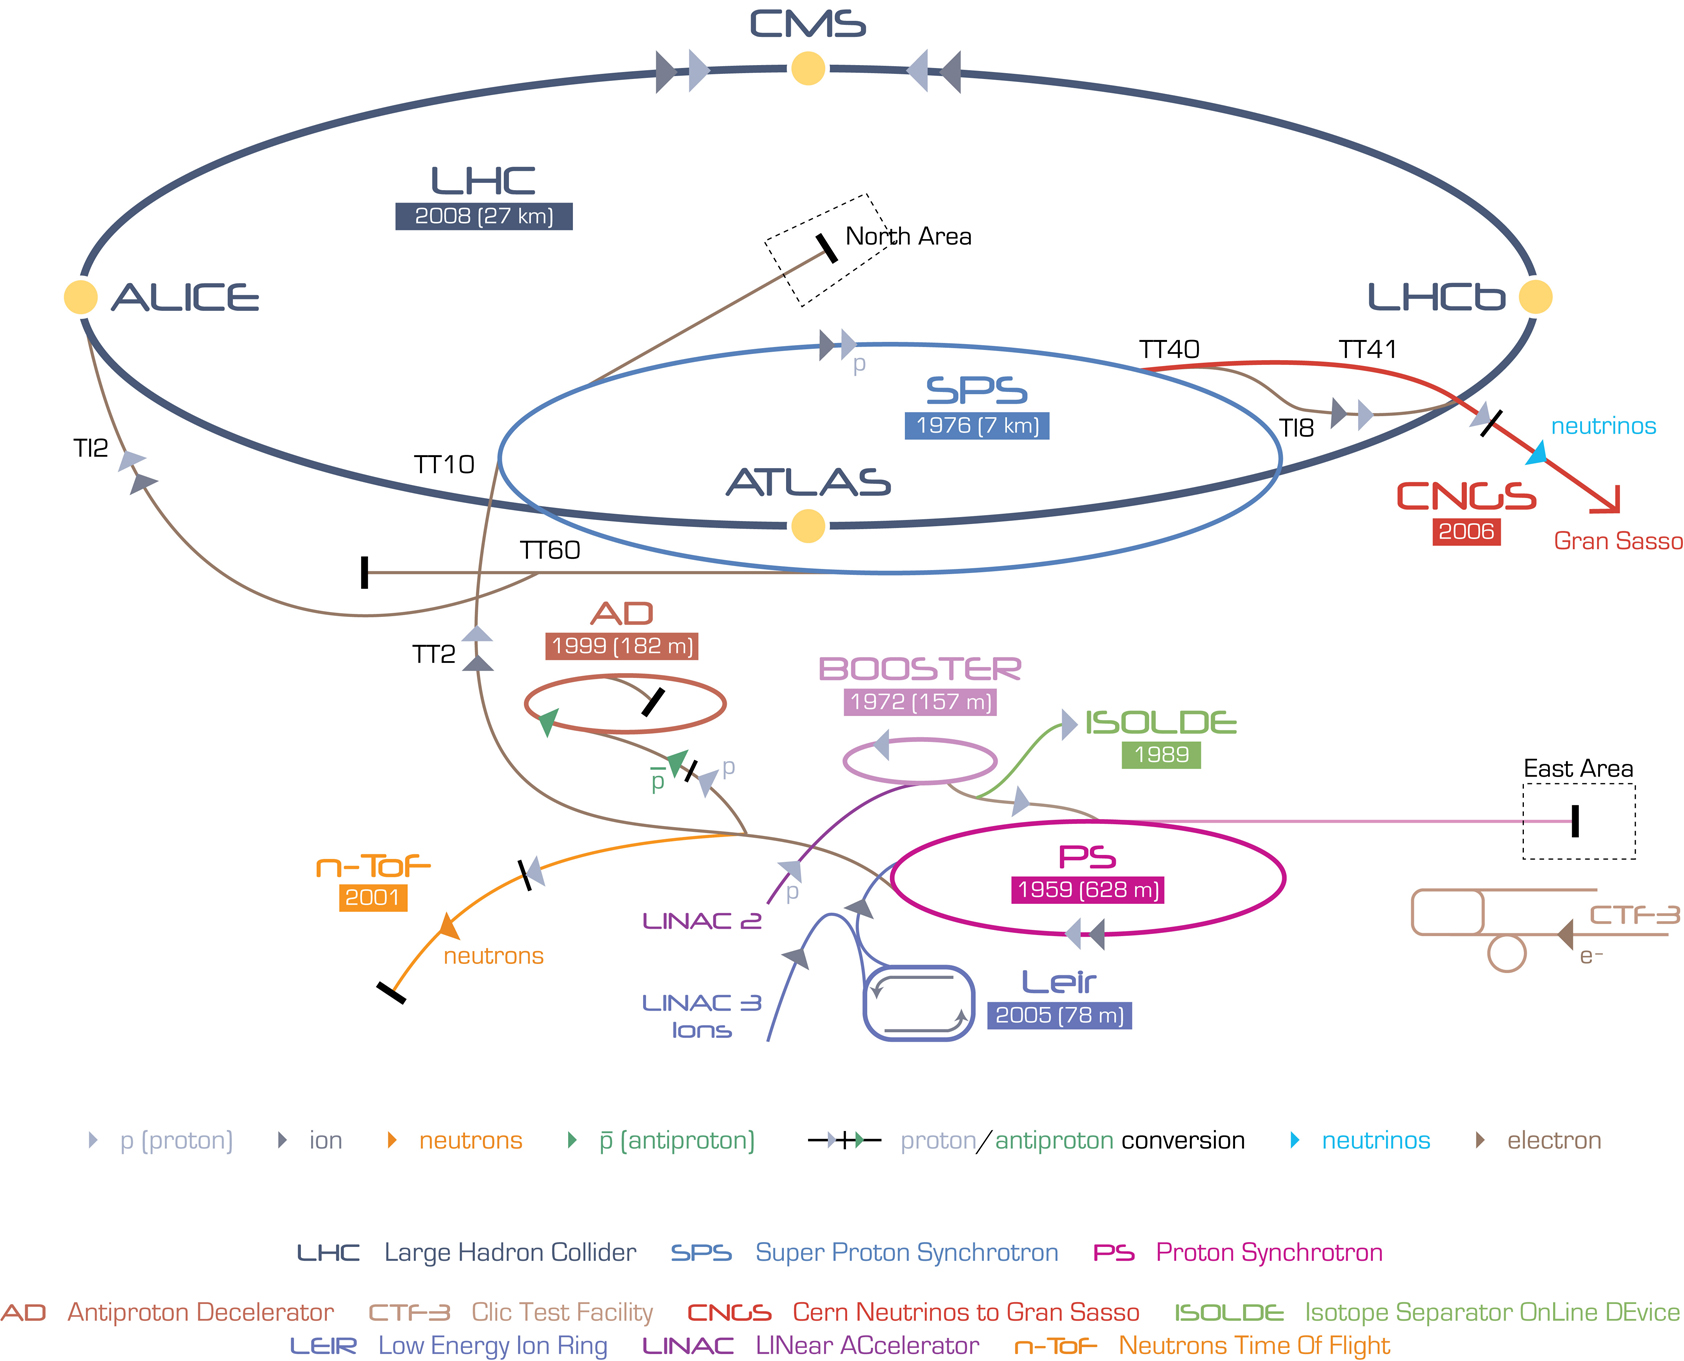
\includegraphics[width=.75\textwidth]{figures/Cern-Accelerator-Complex.jpg}
  \caption{Schema dell'apparato di iniezione e rivelazione nel tunnel di LHC. LHC \`e preposto a molteplici scopi oltre alle collisioni protone-protone, tra cui accelerazione e collisioni tra ioni pesanti (esperimento ALICE), produzione di fasci di neutrini per osservarne le oscillazioni (esperimento CerN to Gran Sasso).}
  \label{fig:LHC_accelerator_complex}
\end{figure}

\noindent Come detto, LHC \`e soltanto la fase terminale di una serie di macchine che accelerano i protoni ad energie crescenti. I protoni vengono estratti da atomi di idrogeno, quindi vengono immessi in un acceleratore lineare, Linac2, che li porta a 50 MeV. Successivamente vengono accelerati in un piccolo sincrotrone, un Booster, che ne aumenta l'energia fino a 1.4 GeV, quindi nel Proton Synchrotron dove arrivano a 25 GeV. Il Super Proton Synchrotron li accelera fino a 450 GeV ed infine essi vengono iniettati nell'anello principale di LHC, dove le cavit\`a a radiofrequenza li porteranno, nominalmente, fino a 14 TeV. Uno schema degli apparati di accelerazione e iniezione \`e mostrato in figura \ref{fig:LHCiniettori}[13].\\%: $http://ab-div.web.cern.ch/ab-div/Publications/LHC-DesignReport.html$]
I fasci, ad LHC, sono suddivisi in pacchetti, necessari per risolvere una delle problematiche che sorgono ai sincrotroni (detta stabilit\`a di fase). Prima della collisione, speciali magneti riducono ciascun pacchetto ad una larghezza di 16 $\mu$m e ad una lunghezza di 80 mm. In ognuno sono presenti circa $10^{11}$ protoni. Presso l'esperimento CMS, secondo il progetto di costruzione, le collisioni avverranno ogni 25 ns (fino ad ora sono avvenute ogni 50 ns), corrispondenti a una frequenza di 40 MHz e ad una luminosit\`a istantanea di $10^{34}\mbox{ cm}^{-2} \mbox{s}^{-1}$. Queste frequenze elevate generano un problema noto con il nome di ``pile-up'', che consiste nel moltiplicarsi del numero di vertici primari di interazione. Ad un medesimo evento registrato prodotto dalle collisioni ogni 50 ns, infatti, corrispondono fino a 30 vertici di interazione; essi aumenteranno a 40 quando si arriver\`a a realizzare una collisione ogni 25 ns.\\
Le quantit\`a di rilevanza per un acceleratore sono l'energia del centro di massa, che definisce la massima energia disponibile negli scontri tra le particelle, corrispondente alla somma delle energie dei singoli fasci, e la luminosit\`a, che descrive invece la frequenza di interazione tra i fasci. Ammettendo che ciascun pacchetto di un fascio contenga $n_1$ protoni e l'altro ne contenga $n_2$, che l'area in cui i pacchetti si urtano sia $\Sigma$ e che la frequenza di rivoluzione attorno all'anello sia $f$, abbiamo che la luminosit\`a istantanea \`e data da:
\begin{equation}
\mathcal{L} = f \frac{n_1 n_2}{\Sigma}.
\end{equation}
Un generico processo i-esimo con sezione d'urto $\sigma_i$ avr\`a allora la frequenza di interazione $R_i$:
\begin{equation}
R_i = \frac{dN_i}{dt}= \sigma_i \mathcal{L},
\end{equation}
mentre il numero di eventi totali registrati nell'intervallo di tempo $(0,\tau)$ si ottiene tramite la luminosit\`a integrata:
\begin{equation}
N_i = \sigma_i \int_0^{\tau} \mathcal{L} dt.
\end{equation}
\subsection{Interazioni protone-protone}

\begin{figure}[!htb]
  \centering
    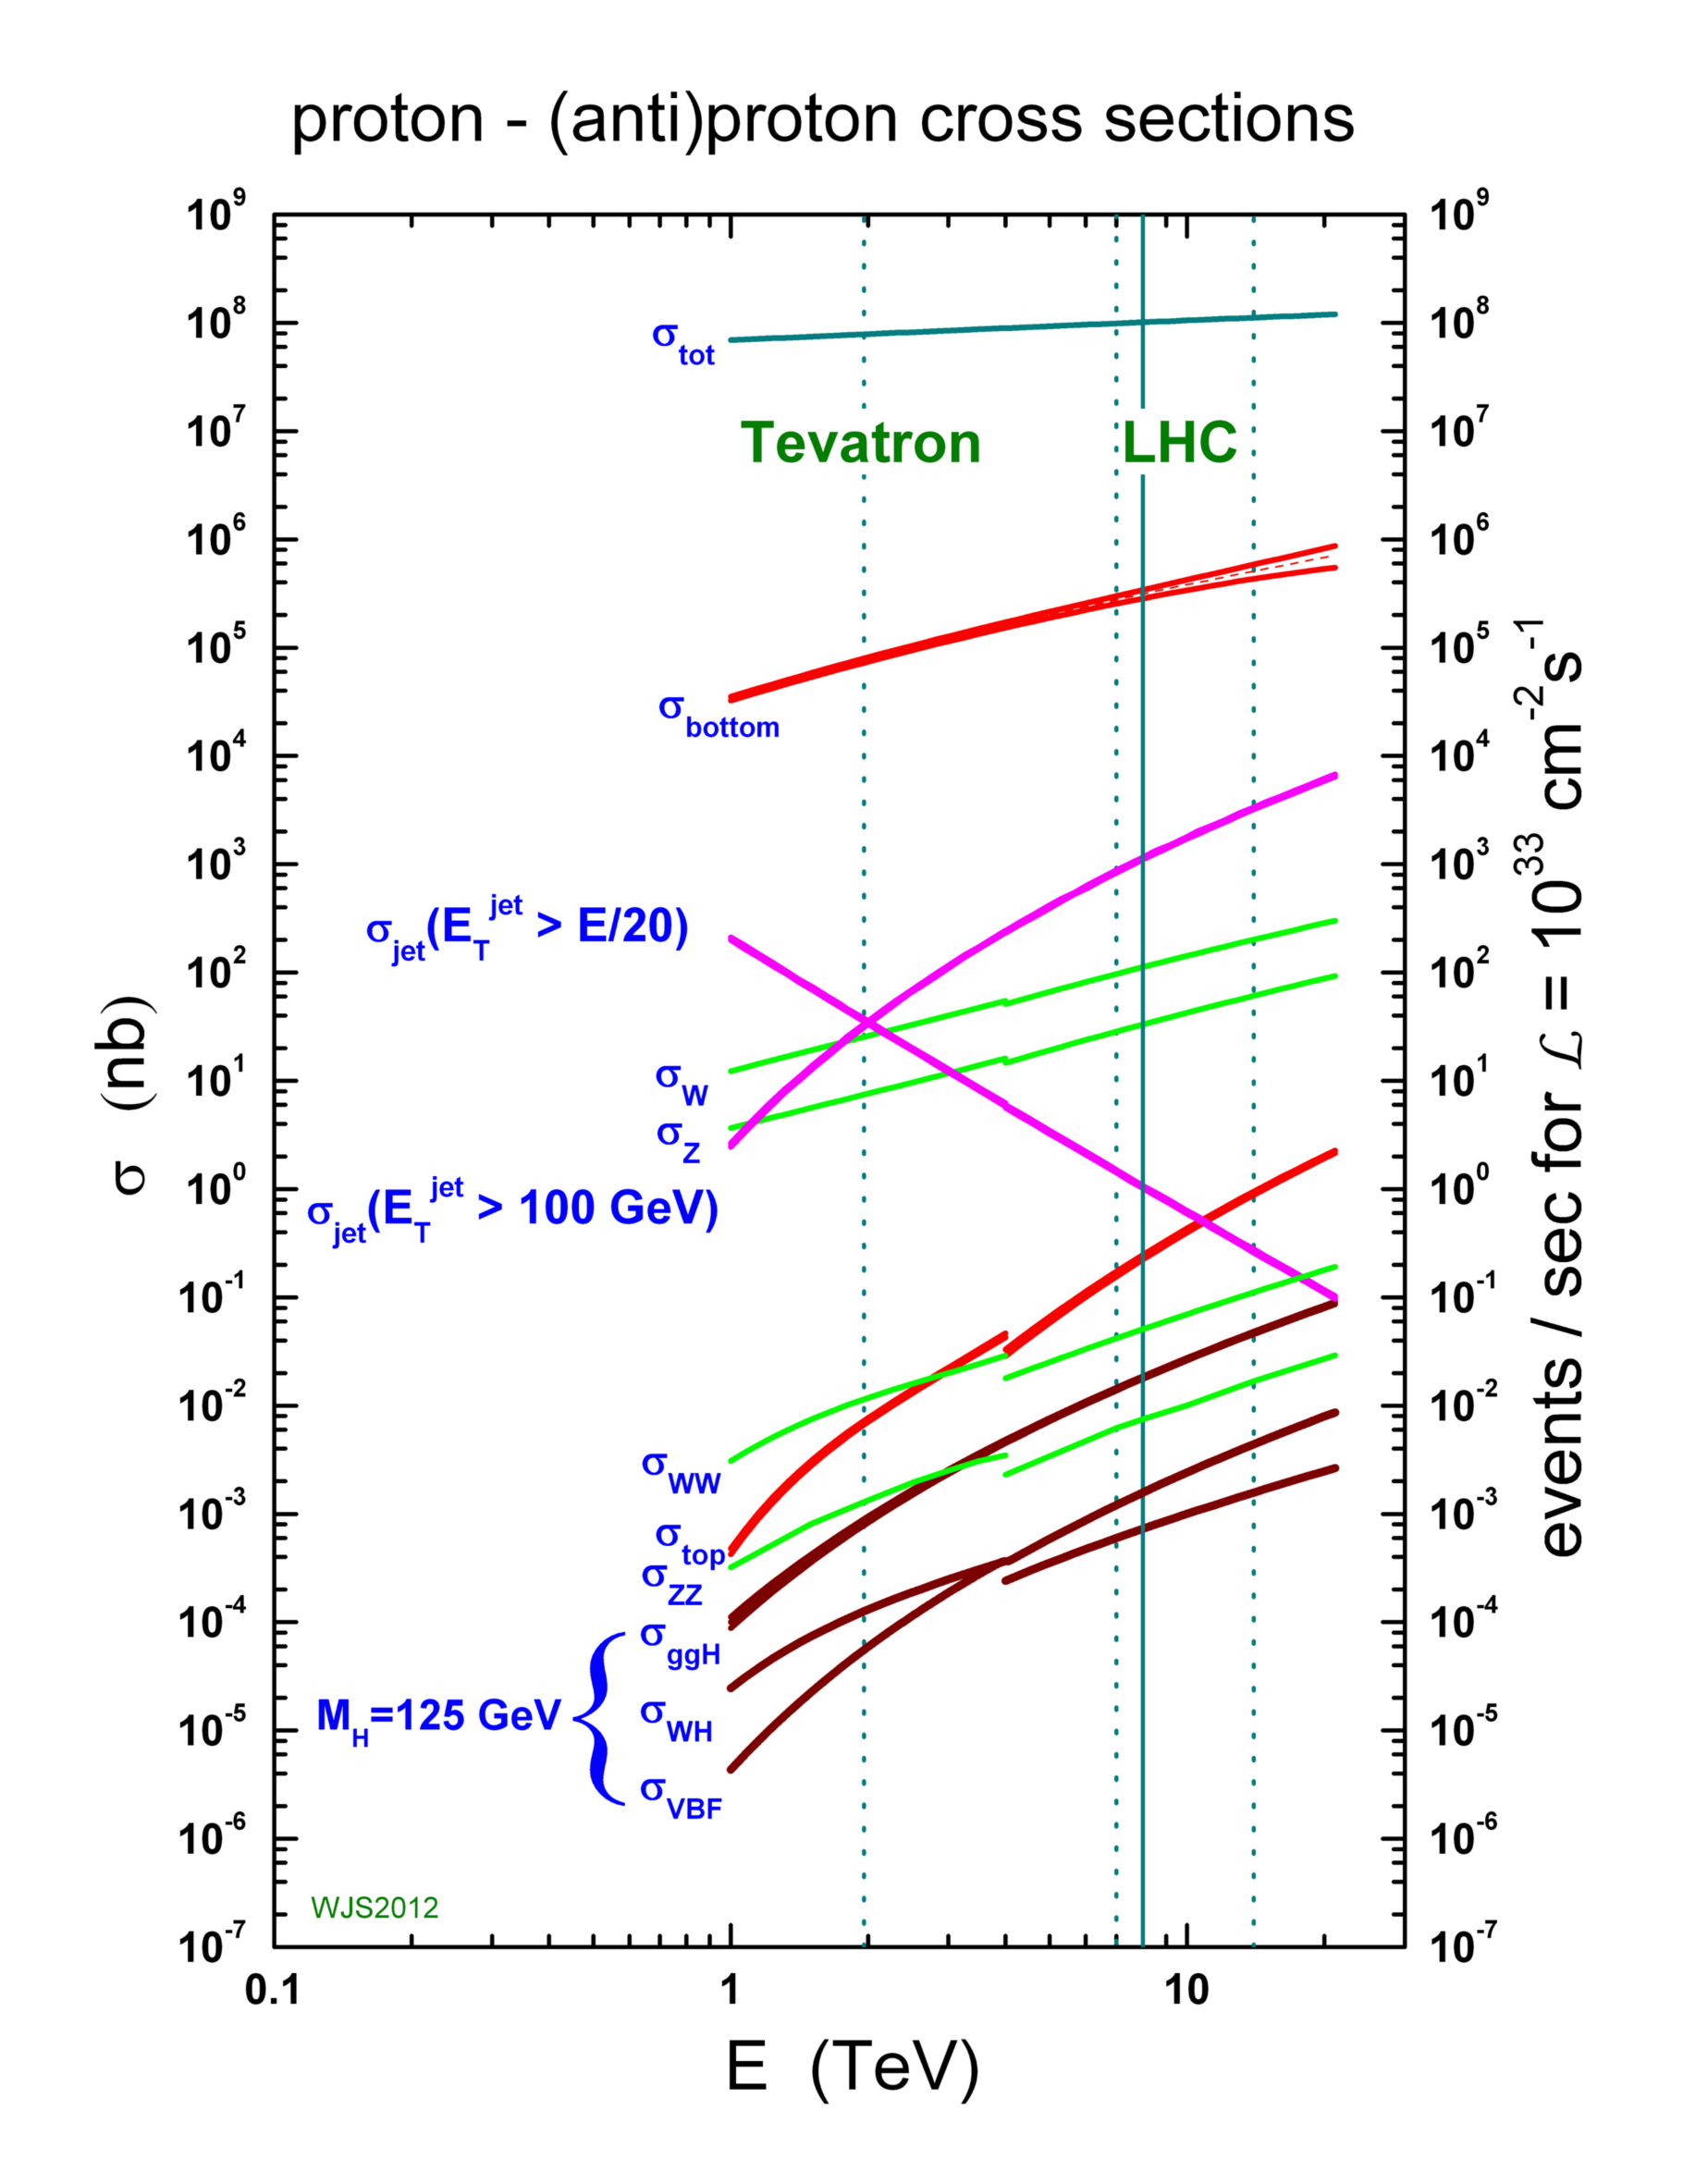
\includegraphics[width=.5\textwidth]{figures/crosssections2013.jpg}
  \caption{Sezioni d'urto e frequenza di eventi attesi da collisioni protone-protone in funzione della massa della particella prodotta (o dell'energia trasversa pi\`u alta dei jets prodotti) per $\sqrt{s}=14$ TeV[14].}
  \label{fig:LHC_pp_cross_section}
\end{figure}

%Figura da CMS Collaboration, DAQ generic figures gallery online at http://cmsdoc.cern.ch/cms/TDR/DAQ/TDRweb/daqgenericjpg.htm
\noindent Nonostante la possibilit\`a di raggiungere luminosit\`a ed energie maggiori, le collisioni tra protoni sono molto pi\`u complesse rispetto a quelle tra leptoni: non soltanto per la proliferazione dei fondi, specialmente da QCD, che rendono molto difficoltoso discriminare il segnale e distinguere i vertici di interazione primari (il loro moltiplicarsi va sotto il nome di {\itshape pileup}), ma anche per l'impossibilit\`a di conoscere con esattezza l'impulso dei partoni che partecipano alla collisione.\\
La maggior parte degli eventi ad LHC sono le interazioni soffici, vale a dire con basso momento trasverso: si tratta tipicamente di urti elastici o difrattivi che non sono di interesse per indagini di nuova fisica. Nei processi detti duri, al contrario, la quantit\`a di momento trasferito \`e elevata: questi eventi sono i pi\`u semplici da distinguere nelle geometrie dei rivelatori e sono quelli in cui vengono prodotte le particelle pi\`u massive.\\
Come \`e noto dalla QCD, ad alti momenti trasferiti \`e lecito trattare un protone come un insieme di partoni, ciascuno dei quali trasporta una frazione $x$ del momento iniziale del fascio e la cui struttura \`e descritta dalle parton distribution function (PDF) $f(x,Q^2)$, funzioni della variabile di Bjorken e del momento trasferito $Q^2$. Nel caso in cui l'energia del centro di massa sia elevata al punto da rendere trascurabili le masse dei singoli oggetti, l'energia effettivamente disponibile per gli urti tra due partoni 1 e 2 \`e una quantit\`a incognita, $\sqrt{x_1 x_2 s}$. La sezione d'urto di un processo partonico generico si pu\`o esprimere sfruttando la fattorizzazione lecita in regime di QCD perturbativa:
\begin{equation}
\sigma = \int dx_1 f_1(x_1,Q^2) \int dx_2 f_2(x_2,Q^2) \sigma_{12}(x_1 p_1, x_2 p_2, Q^2),
\end{equation}
dove $\sigma_{12}$ indica la sezione d'urto elementare del processo partonico ed $f_1,f_2$ sono le PDF. In figura \ref{fig:cross_section} sono rappresentate le sezioni d'urto elementari in funzione della massa della particella prodotta: grazie all'elevata luminosit\`a di LHC \`e possibile osservare fenomeni molto rari mai visti prima, come ad esempio il decadimento del bosone di Higgs in due fotoni o in quattro leptoni, canali nei quali la particella \`e stata scoperta nel 2012.

\section{CMS detector}

Compact Muon Solenoid, installato in una caverna sotterranea nei pressi di Cessy, in Francia, \`e un rivelatore di forma cilindrica, \`e lungo 22 m, ha un diametro di 15 m, una massa di 12500 tonnellate ed \`e preposto a molteplici scopi. La maggior parte dei processi fisici che si vogliono esplorare hanno basse sezioni d'urto, mentre, come \`e ben noto, i prodotti delle collisioni tra protoni sono dominati da elevati fondi QCD: CMS \`e progettato in modo da avere un'elevata capacit\`a di discriminazione degli eventi rari, sfruttando in particolare i canali comprendenti elettroni e muoni, e una grande precisione di misura dei vertici secondari, necessaria per distinguere i $\tau$ e gli adroni contenenti quark pesanti. L'elevata luminosit\`a nominale di LHC, come accennato, comporta il problema del pile-up: questi effetti possono essere ridotti utilizzando rivelatori ad elevata granularit\`a. L'occupazione si abbassa segmentando l'apparato in molti sottogruppi di rivelatori, al costo di dover ottenere un'ottima sincronizzazione tra di essi. L'alta frequenza di interazione, inoltre, necessita un'alta risoluzione temporale. Infine, gli elevati livelli di radiazione attorno al vertice richiedono apparati robusti e resistenti.

\begin{figure}[!htb]
  \centering
    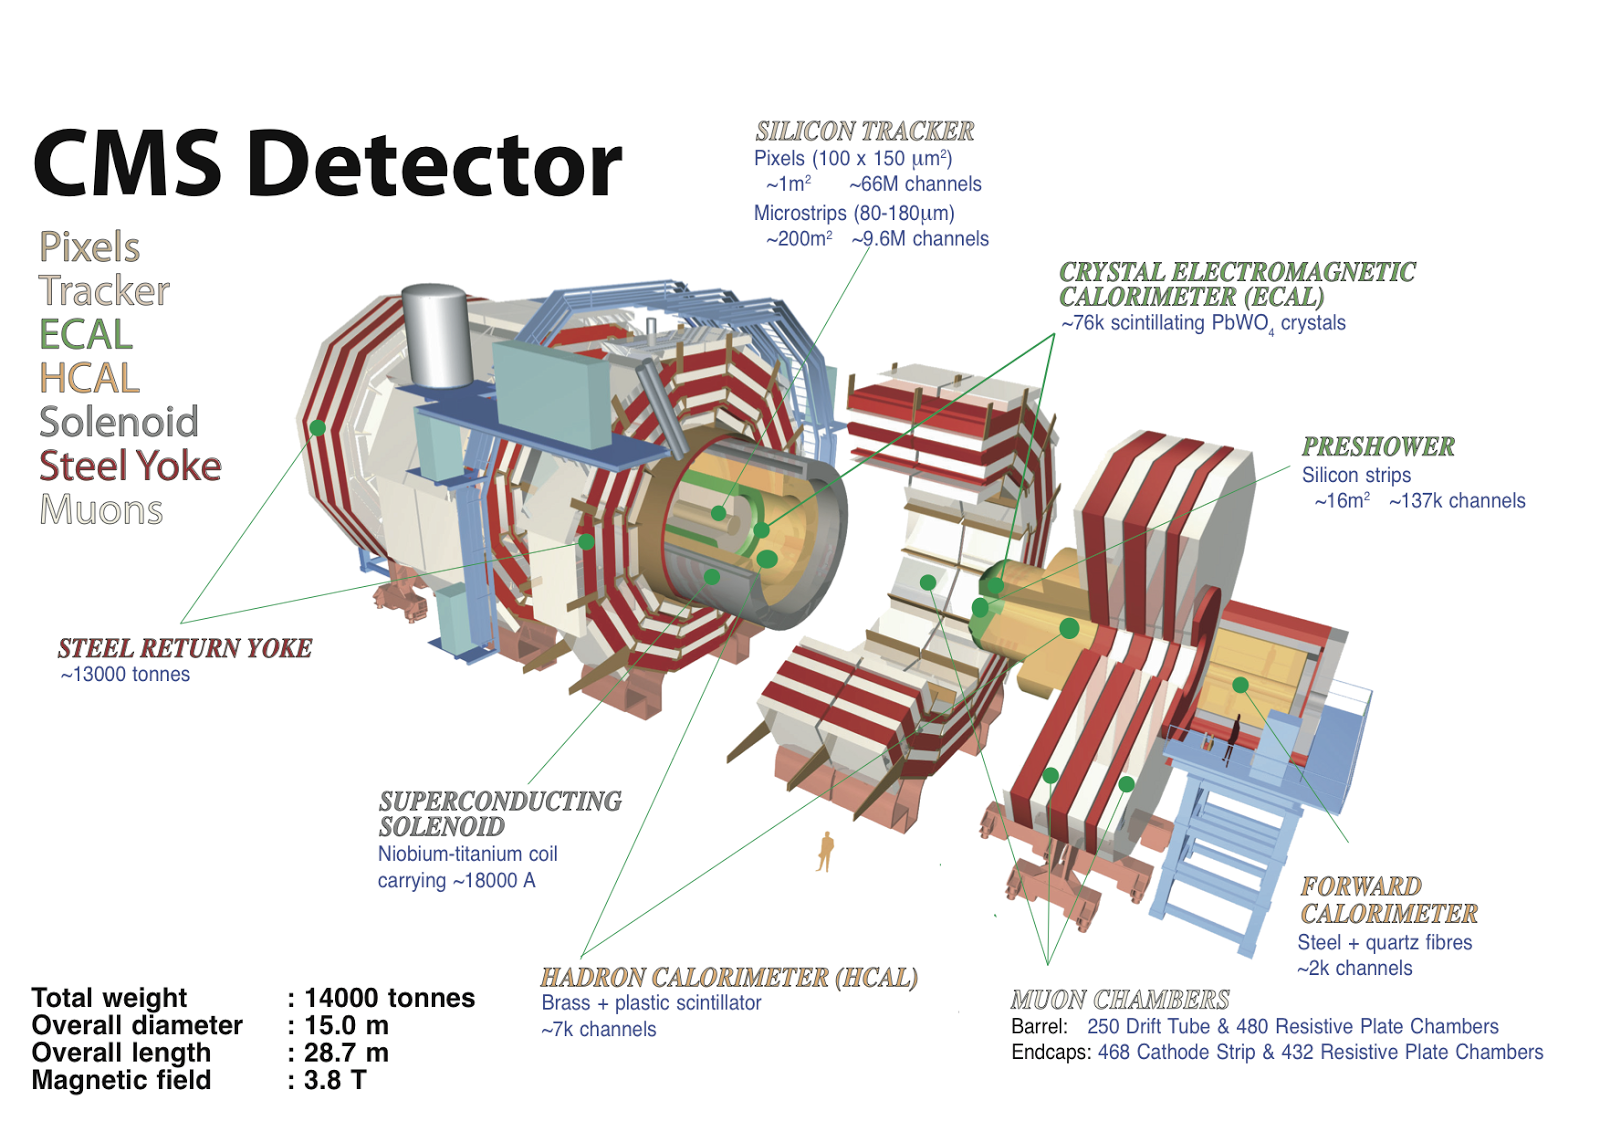
\includegraphics[width=.99\textwidth]{figures/cms_3d.png}
  \caption{Rappresentazione grafica del rivelatore CMS.}
  \label{fig:CMS_1}
\end{figure}

\noindent In figura \ref{fig:CMS_1} \`e rappresentato uno schema dell'esperimento e dei principali gruppi di rivelatori. Prima di passare a descriverne ciascuno nel dettaglio, ponendo particolare attenzione ai tracciatori e al sistema per l'identificazione dei muoni, voglio precisare alcuni termini ricorrenti. Vista la struttura geometrica di CMS, si preferisce chiamare ``barrel'' la superficie laterale del cilindro, ``endcap'' le due basi circolari. I rivelatori ``forward'', disposti oltre gli endcap, servono per coprire un'ulteriore regione geometrica dove la radiazione \`e pi\`u intensa. I rivelatori di traccia al silicio sono spesso chiamati col nome ``tracker''; per il calorimetro elettromagnetico si usa la sigla ECAL; per il calorimetro adronico si usa la sigla HCAL; per il trigger di livello 1 si usa la sigla L1 trigger; per il trigger di alto livello si usa la sigla HLT.\\
La figura \ref{fig:particelle} esemplifica con chiarezza qual \`e la traiettoria che ciascun tipo di particella, mediamente, percorre all'interno di CMS.

\begin{figure}[!htb]
  \centering
    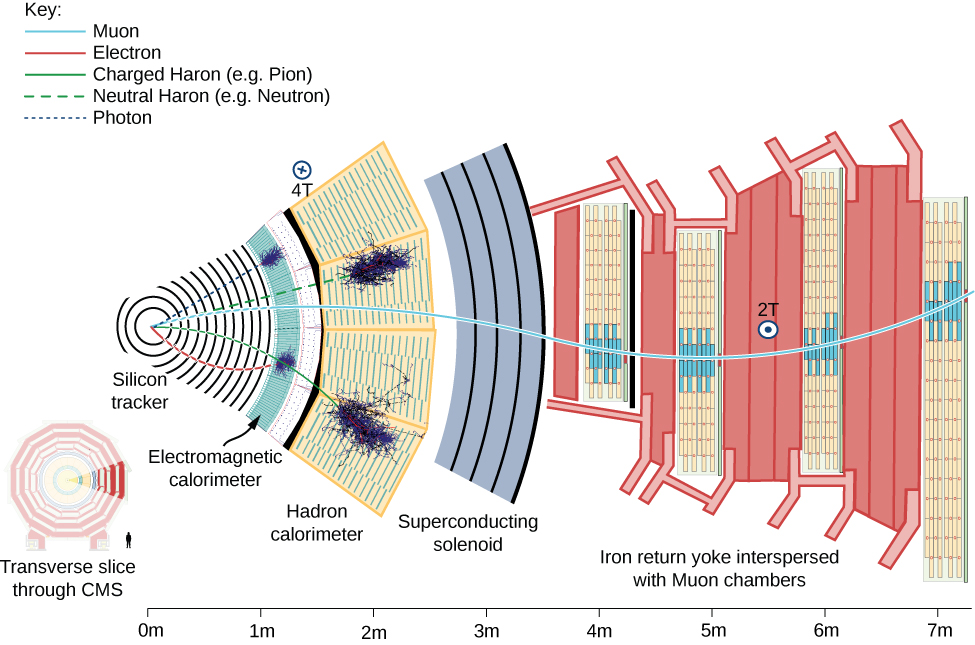
\includegraphics[width=.99\textwidth]{figures/CMS_particles.jpg}
  \caption{Percorso medio di una particella all'interno di CMS. Un muone, in azzurro, attraversa tutti i rivelatori percorrendo una traiettoria curva, lasciando segnale nel tracciatore, nei calorimetri e nelle varie stazioni per i muoni. Un elettrone, in rosso, lascia segnale nei tracciatori e viene assorbito dal calorimetro elettromagnetico. Un fotone, in azzurro tratteggiato, percorre una traiettoria dritta e sciama soltanto nel calorimetro elettromagnetico, senza rilasciare segnale nel tracciatore. Un adrone, in verde (tratteggiato se neutro), lascia segnale nei tracciatori se carico e sciama nel calorimetro adronico.}
  \label{fig:CMS_particles}
\end{figure}

\subsection{Il sistema di coordinate}
Il sistema di coordinate, al quale far\`o spesso riferimento, \`e orientato nel seguente modo. L'asse $\mathrm{x}$, in direzione radiale, punta verso il centro dell'anello di LHC; l'asse $\mathrm{y}$ \`e verticale e punta verso l'alto; l'asse $\mathrm{z}$ \`e lungo la direzione del fascio. L'angolo azimutale, $\Phi$, giace nel piano $\mathrm{xy}$ e si misura a partire dall'asse $\mathrm{x}$; la coordinata radiale in questo piano si indica con $\mathrm{r}$. L'angolo polare $\theta$ \`e definito nel piano $\mathrm{rz}$. La componente del momento trasversa alla direzione del fascio, indicata con $p_T$, si calcola dalle componenti $\mathrm{x}$ ed $\mathrm{y}$. L'energia trasversa \`e definita da $E_T = E \sin{\theta}$.\\
\`E bene introdurre altre due grandezze di comodo utilizzo, la rapidit\`a $y$ e la pseudorapidit\`a $\eta$, definite nei modi seguenti in funzione dell'energia della particella $E$, del suo momento longitudinale lungo l'asse $\mathrm{z}$ e del modulo del momento:
\begin{equation}
y = \frac{1}{2} \log{\frac{E + p_z}{E - p_z}}\\
\end{equation}
\begin{equation}
\eta = \frac{1}{2} \log{\frac{|\bar{p}| + p_z}{|\bar{p}| - p_z}} = -\log{\tan{\frac{\theta}{2}}}.
\end{equation}
Quando la particella \`e emessa in avanti, ossia per $\theta = 0$, $\eta \rightarrow \infty$. Quando la particella \`e emessa trasversalmente al fascio, ossia per $\theta = \pi /2$, $\eta = 0$. Ad energie elevate, quando le masse diventano trascurabili, rapidit\`a e pseudorapidit\`a coincidono. Queste due grandezze vengono ampiamente usate perch\'e sono invarianti per boost di Lorentz lungo la direzione del fascio.

\begin{figure}[!htb]
  \centering
    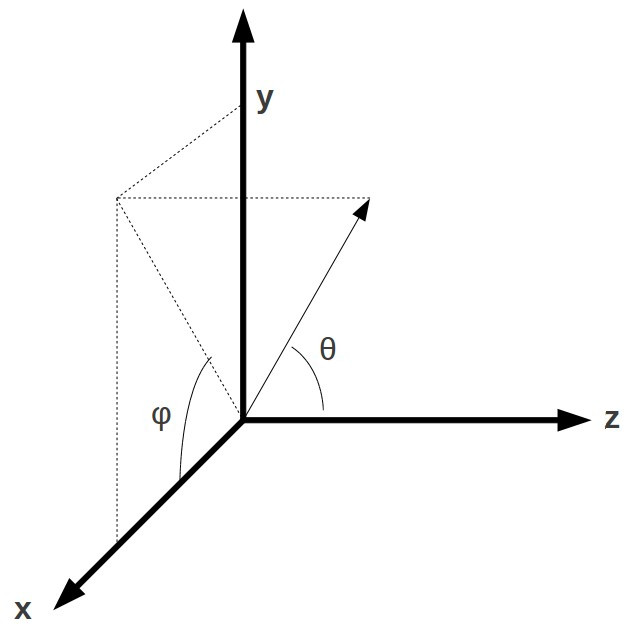
\includegraphics[width=.3\textwidth]{figures/CMS_CoordSys.jpg}
  \caption{Coord sys.}
  \label{fig:CMS_CoordSys}
\end{figure}

\subsection{Il solenoide}
Il grande solenoide superconduttore, un cilindro cavo lungo 13 m e di diametro interno pari a 6 m, fornisce un intenso campo magnetico massimo di 3.8 T, capace di piegare le traiettorie delle particelle cariche per le misure del loro momento $p$, data la relazione tra braccio di leva $R$ e campo magnetico $B$: $p [\text{GeV}] = 0.3 B [\text{T}] R [\text{m}]$. Le linee di campo del magnete sono chiuse da circa 10000 tonnellate di ferro, che costituiscono il giogo di ritorno intervallato alle apparecchiature di rivelazione dei muoni. All'interno dei filamenti di niobio e titanio che generano il campo scorre una corrente elettrica massima di 19 kA; l'energia massima immagazzinata nel solenoide ammonta a 2.6 GJ.
\begin{figure}[!htb]
  \centering
    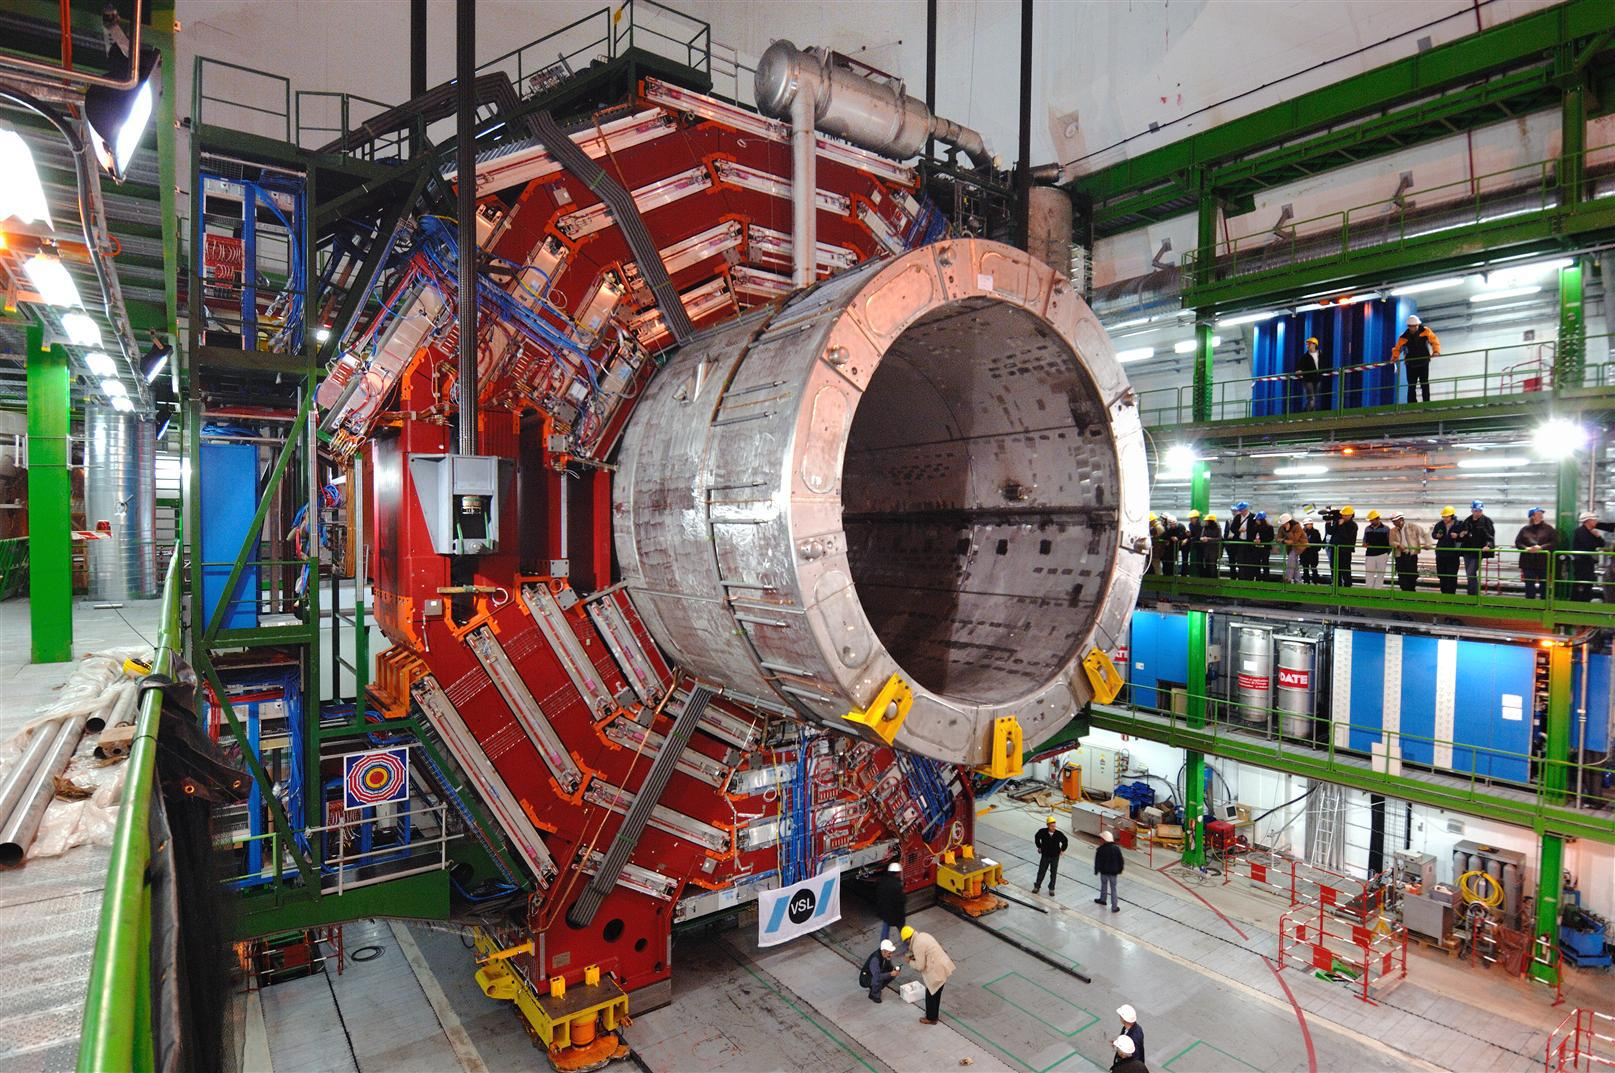
\includegraphics[width=.5\textwidth]{figures/CMS_solenoid.jpeg}
  \caption{Solenoid.}
  \label{fig:CMS_solenoid}
\end{figure}

\subsection{I tracciatori}
Il sistema dei tracciatori a CMS \`e interamente costituito da rivelatori al silicio. La loro elevata precisione nella ricostruzione dei vertici secondari li rende strumenti di vitale importanza per l'identificazione di quark (charm, beauty) e leptoni pesanti ($\tau$), prodotti in numerosissimi processi fisici interessanti.\\
I tracciatori coprono una pseudorapidit\`a $|\eta|<2.5$ per un'area attiva di circa $200\mbox{ m}^2$ e sono suddivisi nel pixel detector, pi\`u vicino al vertice di interazione, e nello strip detector, che copre un raggio compreso tra 0.2 e 1.2 m. L'elevata granularit\`a, come accennato, permette di abbassare l'occupazione, vale a dire di avere meno eventi per ciascun sotto-rivelatore: i pixel hanno un'area di $100 \times 150 \mbox{ }{\mu{m}}^2$ e uno spessore di 285 $\mu$m. Le strip adoperate a raggi intermedi (20-55 cm) hanno dimensioni 10 cm $\times$ 80 $\mu$m $\times$ 320 $\mu$m; quelle a raggi maggiori (55-110 cm) 25 cm $\times$ 180 $\mu$m $\times$ 500 $\mu$m. In totale ci sono 1440 moduli di pixel per un totale di 66 milioni di canali di lettura, e 15148 moduli di strip per un totale di 9.3 milioni di canali di lettura.\\
L'altissima frequenza degli eventi implica l'utilizzo di un'elettronica capace di leggere molto rapidamente i segnali, portando ad un elevato consumo energetico: questo richiede un efficace sistema di raffreddamento che mantenga il rivelatore ad una temperatura di $\approx10^{\circ}$ C in modo da preservarne la durata.\\
Il pixel detector \`e costituito da tre strati di rivelatori nel barrel e da due dischi agli endcaps. I moduli nel barrel sono disposti parallelamente al campo magnetico, mentre agli endcaps sono inclinati di circa $20^{\circ}$: le coppie elettrone-lacuna prodotte nel semiconduttore sono allora soggette ad una forza di Lorentz e il loro moto di deriva non avviene pi\`u lungo le linee del campo elettrico, bens\`i esse si sparpagliano lungo diversi pixel. Calcolando il centro della distribuzione di carica raccolta, \`e possibile determinare la posizione della particella carica che ha attraversato il rivelatore con una risoluzione di 15 $\mu$m, sia nel piano $\mathrm{r}\Phi$, sia lungo $\mathrm{z}$.\\
Il tracciatore a strip \`e composto da quattro sotto-sistemi: il tracker inner barrel, diviso in 4 strati; il tracker outer barrel, in 6 strati; il tracker inner disk, in 3 strati; il tracker endcaps, in 9 strati. I moduli pi\`u esterni, sia del barrel che dell'endcap, sono leggibili sia dal fronte che dal retro.\\
\begin{figure}[!htb]
  \centering
    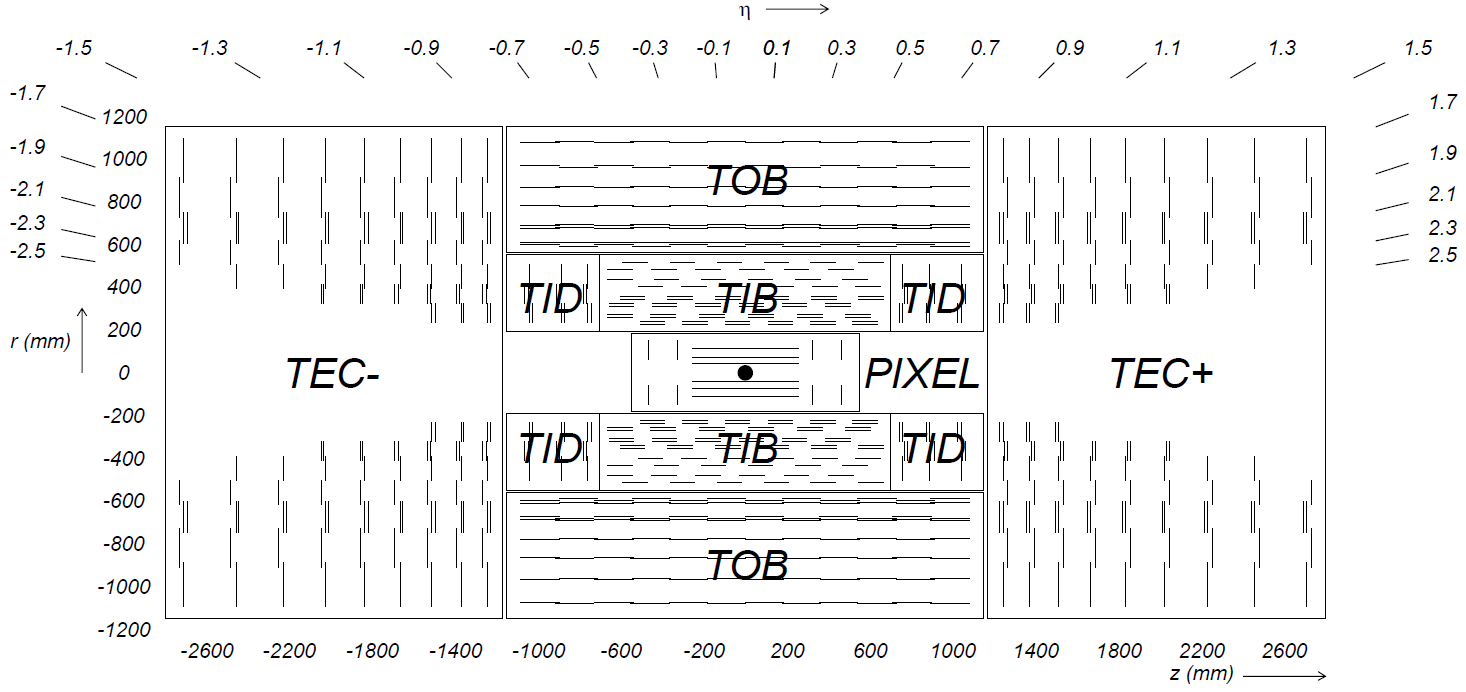
\includegraphics[width=.9\textwidth]{figures/cmstracker.png}
  \caption{Tracker.}
  \label{fig:CMS_tracker}
\end{figure}
%Nel capitolo 4 descriver\`o le tecniche di ricostruzione delle tracce nei rivelatori al silicio, in particolare dei muoni.\\
%L'efficienza di ricostruzione delle tracce dei muoni \`e stata misurata essere attorno al 99\%, essa cala drasticamente per $|\eta|>2.1$ a causa della ridotta copertura geometrica del pixel detector. Le efficienze di rivelazione degli adroni sono tipicamente pi\`u basse perch\'e interagiscono con il materiale. La risoluzione in $p_T$, sempre per i muoni, \`e attorno all'1-2\% per $|\eta|>1.6$ e per momenti elevati; a momenti pi\`u bassi dominano effetti di scattering multiplo e dipendono dalla quantit\`a di materiale attraversato.\\

\subsection{Il calorimetro elettromagnetico}
Il calorimetro elettromagnetico di CMS \`e un rivelatore omogeneo composto da cristalli scintillatori di tungstenato di piombo ($\mbox{PbWO}_4$), ideali per le misure di fotoni ed elettroni. Il calorimetro \`e suddiviso in due gruppi di sotto-rivelatori, uno nel barrel ed uno per ciascun endcap; nel complesso copre una regione geometrica fino ad $|\eta|<3$. Il $\mbox{PbWO}_4$ \`e stato scelto perch\'e permette una risposta temporale rapida (in 25 ns, ad ogni collisione tra pacchetti, viene emesso l'85\% della luce di scintillazione), ha elevate efficienza di scintillazione e resistenza alla radiazione. I 61200 cristalli impiegati nella regione di barrel hanno dimensioni $(22 \times 22) \mbox{ mm}^2 \times 23 \mbox{ cm}$, per una corrispondente lunghezza di radiazione di $25.8 X_0$; i 7324 cristalli negli endcaps hanno dimensioni $ 28.6 \times 28.6 \mbox{ mm}^2 \times 22 \mbox{ cm}$, per una corrispondente lunghezza di radiazione di $24.7 X_0$. Prima della regione di endcaps, \`e disposto un rivelatore di preshower costituito da due strati di sandwich piombo/silicio, per una lunghezza di radiazione di $3X_0$: questo permette una maggiore efficienza di rivelazione nella regione in avanti e permette di utilizzare cristalli pi\`u piccoli agli endcaps; \`e stato installato appositamente per distinguere due fotoni dal decadimento del $\pi_0$ e per poter indagare il canale di decadimento raro dell'Higgs $H \rightarrow \gamma \gamma$.\\
La luce scintillata nel barrel viene raccolta e amplificata da dei fotodiodi a valanga; agli endcaps, dove la frequenza degli eventi \`e pi\`u alta, il segnale \`e letto da fototridiodi a vuoto. La raccolta e l'amplificazione della radiazione da scintillazione \`e fortemente dipendente dalla temperatura, rendendo necessario un sistema di controllo e raffreddamento ad acqua che mantenga il calorimetro a $18^{\circ}$ C costanti.

\begin{figure}[!htb]
  \centering
    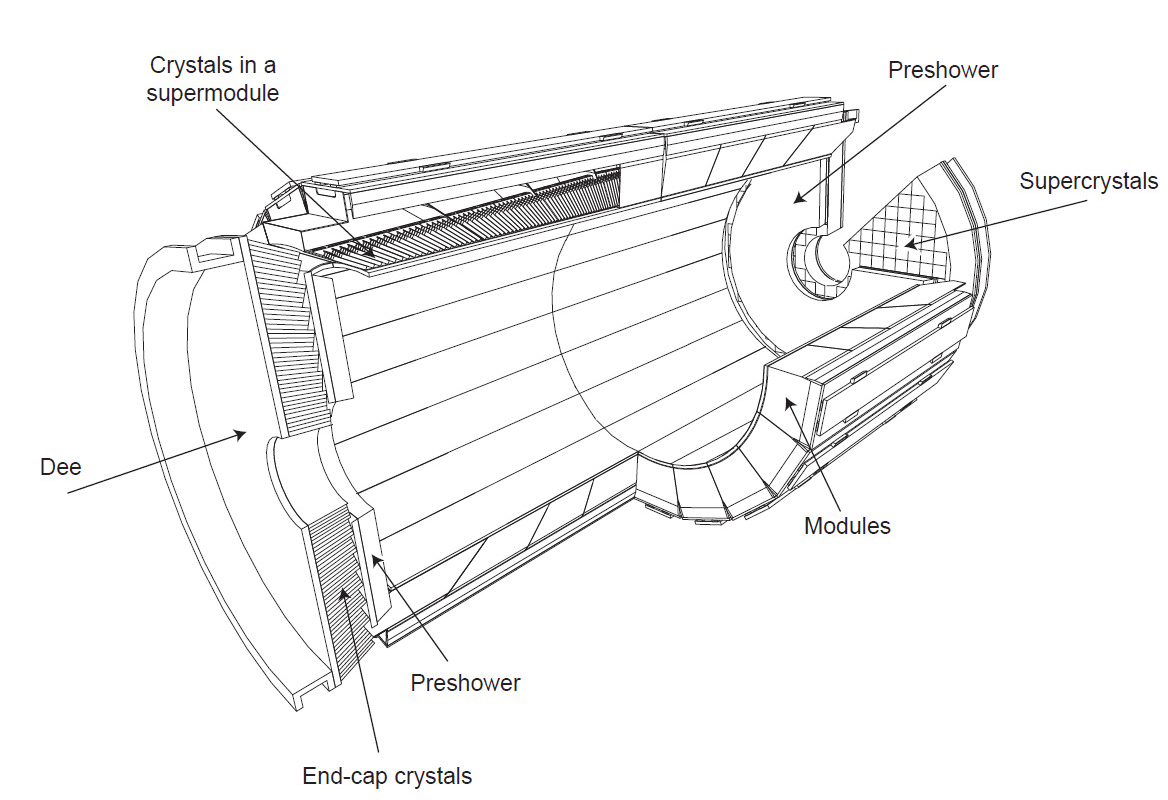
\includegraphics[width=.7\textwidth]{figures/cmsecal.png}
  \caption{Ecal.}
  \label{fig:CMS_ecal}
\end{figure}

\begin{figure}%{l}{0.5\textwidth}
\centering
%\includegraphics[scale=0.3]{risoluzione_ECAL.png}
\caption{Risoluzione in energia di ECAL in funzione dell'energia del fascio di elettroni utilizzato per le misure. Sono mostrati anche i valori per i parametri di fit[16].}
\label{fig:risoluzione_ECAL}
\end{figure}

\noindent La risoluzione in energia del calorimetro \`e parametrizzata secondo l'espressione seguente:
\begin{equation}
{\left( \frac{\sigma}{E} \right)}^2 = {\left( \frac{S}{\sqrt{E}} \right)}^2 + {\left( \frac{N}{E} \right)}^2 + C^2,
\end{equation}
dove $S$ \`e il termine stocastico, $N$ il contributo dal rumore, $C$ un termine costante (contiene le dipendenze dalla calibrazione). In figura \ref{fig:risoluzione_ECAL} sono mostrati i risultati ottenuti da misure di prova con un fascio di elettroni: le stime ottenute sono $S=0.028 \mbox{ GeV}^{\frac{1}{2}}$, $N=0.12 GeV$, $C=0.003$.

\subsection{Il calorimetro adronico}
Il calorimetro adronico \`e costruito a strati alterni di ottone e di scintillatore plastico. La qualit\`a della misura dipende dalla granularit\`a del rivelatore, dalla sua ermeticit\`a e dalla frazione di energia depositata dagli adroni che il calorimetro \`e in grado di rivelare, quindi deve essere spesso abbastanza da assorbire tutti gli sciami adronici. L'estensione radiale del rivelatore nella regione di barrel \`e per\`o limitata dalla presenza dell'ECAL e del solenoide superconduttore: per raggiungere una lunghezza di assorbimento sufficiente (11.8$\lambda$) \`e stato installato un ulteriore strato calorimetrico al di fuori del magnete.\\
La luce di scintillazione, tipicamente nella parte blu-violetta dello spettro elettromagnetico, \`e interpretata da fibre (``wavelenght shifter'') che ne spostano la lunghezza d'onda al verde e la trasportano fino a fotorivelatori ibridi. I primi strati di scintillatore sono disposti immediatamente a ridosso dell'ECAL, mentre gli ultimi a contatto con le camere per i muoni, permettendo cos\`i di raccogliere tutta l'informazione possibile.\\
La risoluzione energetica combinata dei due calorimetri \`e data da:
\begin{equation}
\left( \frac{\sigma}{E} \right) \approx \frac{100\%}{\sqrt{E}} \oplus 45\%.
\end{equation}
Le regioni di barrel e di endcaps dell'HCAL coprono un intervallo di $|\eta|<3$; il calorimetro ``forward'' aggiuntivo arriva fino ad $|\eta|<5.2$. Esso si trova a 11.2 m dal punto di interazione ed \`e stato progettato appositamente in previsione del raggiungimento dell'energia massima di 14 TeV: si calcola infatti che il deposito energetico medio di un adrone prodotto in collisioni $pp$ in queste condizioni sia di 760 GeV nella direzione in avanti, da confrontare con i 100 GeV medi delle altre regioni geometriche. Il calorimetro ``forward'' \`e composto da strati assorbitori di acciaio spessi 55 mm in cui sono innestate delle fibre di quarzo, che agisce da mezzo attivo poich\'e rivela la luce Cherenkov emessa dalle particelle cariche dello sciame, principalmente quella della componente elettromagnetica. La segmentazione longitudinale permette di distinguere i segnali lasciati dagli adroni rispetto a quelli lasciati da elettroni e fotoni.

\begin{figure}[!htb]
  \centering
    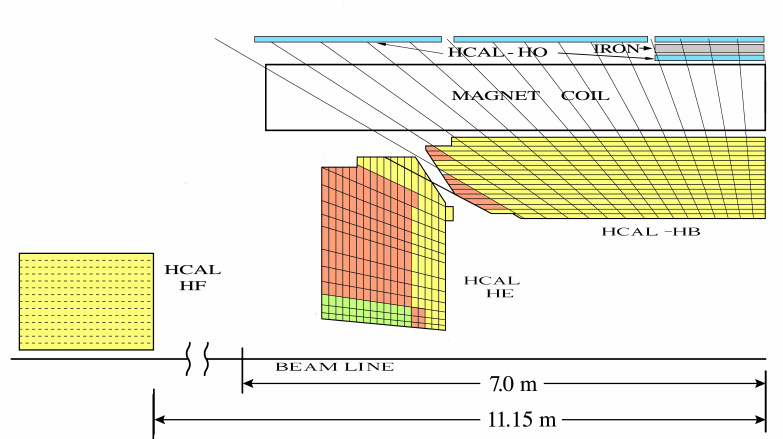
\includegraphics[width=.7\textwidth]{figures/cmshcal.png}
  \caption{Hcal.}
  \label{fig:CMS_hcal}
\end{figure}

\subsection{Sistema per l'identificazione dei muoni}

\begin{figure}[!htb]
  \centering
    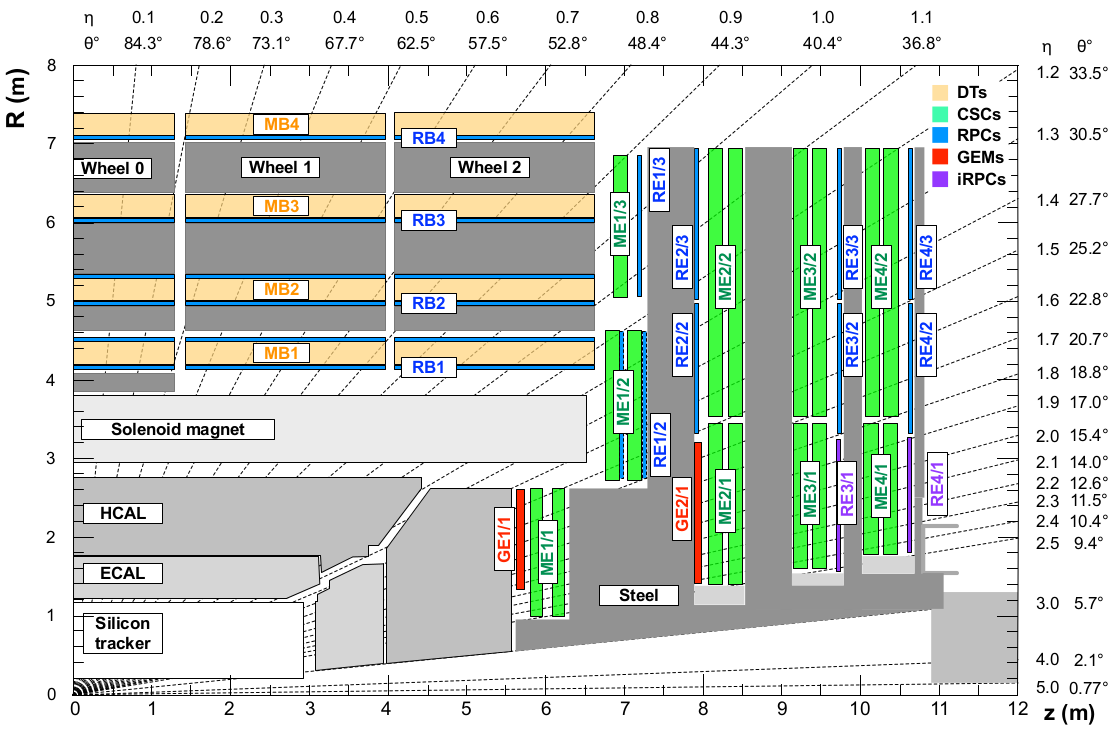
\includegraphics[width=.9\textwidth]{figures/cmsmuon.png}
  \caption{Mu.}
  \label{fig:CMS_muon}
\end{figure}

\begin{figure}%{l}{0.5\textwidth}
\centering
%\includegraphics[scale=0.4]{camere_muoni.png}
\caption{Sezione di CMS fatta parallelamente alla linea del fascio, nel piano $\mathrm{rz}$. Si osservi in particolare la disposizione delle camere a muoni nel barrel (MB) e nell'endcap (ME).}
\label{fig:camere_muoni}
\end{figure}

\noindent L'ultimo gruppo di rivelatori di CMS consiste in una serie di rivelatori a gas per l'identificazione dei muoni, intervallati agli strati di ferro che chiudono le linee del campo magnetico generato dal solenoide. Nel barrel, le stazioni per i muoni sono separate in quattro cilindri concentrici; negli endcaps sono organizzate in tre dischi, ciascuno contenente quattro stazioni. Si pu\`o vedere la loro disposizione in figura \ref{fig:camere_muoni}.\\
Nella regione di barrel, dove ci sono meno muoni e meno neutroni di fondo e dove il campo magnetico \`e meno intenso, vengono utilizzate delle camere con tubi a deriva (DT, drift tube). Agli endcaps, dove i flussi sono maggiori, ci sono delle camere a strip catodici (CSC, cathode strip chambers), che permettono una risposta pi\`u rapida, una maggiore granularit\`a e resistenza agli alti livelli di radiazione. Inoltre, dei rivelatori resistivi (RPC, resistive plate chamber) vengono sfruttati come ulteriore sistema di trigger indipendente per i muoni. In totale sono installati 250 DT, 540 CSC, 610 RPC.

\begin{figure}%{l}{0.5\textwidth}
\centering
%\includegraphics[scale=0.3]{DT.jpg}
%\caption{Schema di una cella elementare nei Drift Tubes. Le tensioni tipicamente applicate sono: +3600 V al filo anodico, +1800 V alle strip di elettrodi, -1200 V ai catodi di alluminio.}
\label{fig:DT}
\end{figure}

\begin{itemize}
\item Ogni cella DT, di dimensioni di $42 \times 13 \mbox{ mm}^2$, contiene una miscela di gas (85\% Ar e 15\% $\mbox{CO}_2$), un filo anodico a carica positiva e due strisce catodiche di alluminio (si veda la figura \ref{fig:DT}) che separano una cella dall'altra. Un piano di celle \`e isolato dall'altro mediante materiale plastico. L'anodo \`e realizzato da un filo di acciaio di 50 $\mu$m posto al centro della cella; in totale a CMS sono montati circa 195000 fili. La distanza della traccia dal filo \`e misurata dal tempo di deriva degli elettroni indotti dalla ionizzazione del gas: due strisce di elettrodi posizionate su due superfici della cella hanno l'obiettivo di dare forma al campo in modo da rendere la velocit\`a di deriva quanto pi\`u uniforme possibile. La risoluzione spaziale complessiva del sistema \`e di 180 $\mu$m. Ogni camera con tubi a deriva (indicata con MB nella figura \ref{fig:camere_muoni}) ha una superficie di circa $2 \times 2.5 \mbox{ m}^2$ e contiene 12 strati di celle DT, arrangiate in tre gruppi di quattro. Il gruppo di celle di mezzo, i cui fili anodici sono disposti perpendicolarmente alla linea di fascio, misura la coordinata $\mathrm{z}$, i due gruppi esterni, in cui i fili anodici sono paralleli al fascio, misurano la coordinata nel piano $\mathrm{r}\Phi$. Le camere di diverse stazioni sono sovrapposte in modo da coprire tutta la coordinata $\Phi$.\\
\item Le CSC sono delle camere proporzionali a molti fili di forma trapezoidale. Sono costituite da 6 piani con i fili anodici attraversati da 7 pannelli con strip catodiche di rame, tutto immerso in una miscela di gas. I fili anodici misurano la coordinata radiale $\mathrm{r}$; le strisce catodiche sono disposte a $\Phi$ costante: interpolando la carica indotta nelle strip \`e possibile ricostruire anche la coordinata azimutale. Come nel caso dei DT, anche le CSC sono sovrapposte in modo da coprire tutta la coordinata $\Phi$. A ciascun endcap ci sono 4 stazioni di CSC che arrivano ad una regione geometrica di $|\eta|<2.4$. Per $0.9<|\eta|<1.2$, un muone attraversa sia i DT del barrel che le CSC degli endcaps. Le CSC di CMS contengono, nel complesso, un volume di gas maggiore di 50 $\mbox{m}^3$ e pi\`u di 2 milioni di fili. Le CSC pi\`u grandi hanno dimensioni massime di 3.4 m lungo la direzione dei catodi e 1.5 m lungo la direzione dei fili anodici. La risoluzione raggiungibile alla massima tensione \`e di circa 80 $\mu$m.\\
\item Gli RPC sono dei piatti plastici ad alta resistivit\`a, separati da un volume riempito di gas, e caricati a tensioni elevate, in modo da lavorare nel regime di ionizzazione a valanga. I piatti sono provvisti di strisce di lettura che raccolgono il segnale al passaggio del muone attraverso il gas. La loro risoluzione spaziale \`e molto bassa, circa 1-2 cm; al contrario la loro rapida risposta temporale (2-3 ns) e l'alta risoluzione (circa 1 ns) li rendono strumenti ideali per il trigger e per la misura del tempo a cui avviene l'interazione. Nel barrel sono montati 6 strati di RPC, negli endcaps ne sono montati 3.\\
\end{itemize}
L'intero sistema misura in maniera ``standalone'' l'impulso con una risoluzione in $p_T$ di circa $\Delta p_T/p_T \approx 8-15\%$ per muoni di $p_T = 10$ GeV/c e di $\Delta p_T/p_T \approx 20-40\%$ per muoni di $p_T = 1$ TeV/c. Combinando con la misura nei rivelatori al silicio la risoluzione passa rispettivamente all'$1\%$ e al $7-16\%$.\\
Vista l'importanza dei muoni per il lavoro di tesi, nel prossimo capitolo illustrer\`o nel dettaglio le tecniche utilizzate per la ricostruzione del segnale.
\subsection{Altri rivelatori}
Tracciatori e camere per i muoni coprono una regione di $|\eta|<2.5$, gli apparati calorimetrici arrivano fino ad $|\eta|<5.2$. Ci sono altri due rivelatori che permettono misure nella regione $5 \leq |\eta| \leq 11$, TOTEM e CASTOR. TOTEM sfrutta dei rivelatori a gas per le misure di scattering elastico protone protone in funzione del loro momento. CASTOR \`e un calorimetro elettromagnetico ed adronico che raccoglie luce Cherenkov, serve per misure di QCD in collisioni p-p, p-ione, ione-ione.
\subsection{Sistema di trigger}
Il sistema di trigger di CMS \`e stato realizzato in funzione delle elevate luminosit\`a e frequenza di interazione; deve essere efficiente nello studio di fenomeni rari e molto diversi da loro, e deve applicare delle selezioni in modo da abbassare la frequenza degli eventi da 40 MHz a circa 100 Hz, tali da consentire la registrazione software. Esso deve inoltre avere tempi decisionali molto brevi, dal momento che ogni 25 ns avviene una collisione: questo intervallo temporale \`e troppo ristretto anche solo per poter leggere i dati raccolti dal rivelatore. Il problema viene superato operando le selezioni in fasi successive, in ciascuna delle quali vengono prese delle decisioni sulla base di una sola parte dei dati. Il trigger di livello 1, L1, \`e un dispositivo elettronico hardware che permette di scende con la frequenza all'ordine di 100 kHz; il trigger di livello alto, HLT, \`e invece basato su algoritmi software capaci di rielaborare il segnale, ed \`e a sua volta separato in due livelli logici (Level-2 e Level-3).\\
\subsubsection{Il trigger di livello 1}
Il trigger L1 ha accesso solamente alle informazioni provenienti dai calorimetri e dalle camere per i muoni. Esso \`e segmentato in pi\`u processi in parallelo, ciascuno dei quali impiega singolarmente meno di 25 ns. La decisione complessiva del L1 viene presa ogni 3.2 $\mu$s, tenendo conto anche dei tempi tecnici per il trasporto del segnale ai dispositivi: questo significa che la parte puramente computazionale deve impiegare meno di 1 $\mu$s.\\
Il trigger di livello 1 \`e suddiviso in tre sistemi: il trigger calorimetrico, il trigger muonico, a sua volta diviso in tre sotto-sistemi indipendenti per ciascuna categoria di rivelatori (DT, RPC, CSC) e il trigger globale, che combina i risultati dei precedenti. Lo scopo del trigger muonico, in particolare, \`e quello di identificare i muoni, ricostruirne la posizione e assegnarne delle variabili relative al punto di collisione. Avere tre sottosistemi differenti permette di combinarne i rispettivi vantaggi: l'elevata risoluzione spaziale (dei DT e delle CSC) e l'eccellente risoluzione temporale (degli RPC).\\
I trigger, pi\`u che operare delle vere e proprie decisioni autonome, hanno l'obiettivo di identificare dei precisi oggetti: elettroni/fotoni e muoni isolati o non isolati, jets centrali, in avanti o provenienti da $\tau$. I quattro candidati migliori di ciascuna categoria vengono mandati al trigger globale insieme a: una misura della loro posizione, momento trasverso e ad un'etichetta che ne identifica la qualit\`a; informazioni di energia trasversa totale e mancante dal trigger calorimetrico; un importante controllo sull'attivit\`a nella regione calorimetrica, che pu\`o essere o meno compatibile con il deposito di energia lasciato dal passaggio di un muone. A questo punto il trigger globale opera le selezioni necessarie, scegliendo uno o pi\`u oggetti che abbiano energia o momento sopra a una determinata soglia; si possono aggiungere richieste sulla geometria, fino ad un massimo di 128 condizioni in parallelo. I trigger pi\`u semplici si basano solitamente sulla presenza di un solo oggetto che abbia $p_T$ o $E_T$ sopra ad una certa soglia (trigger ``single-object''), oppure sulla presenza di due oggetti (trigger ``di-object''), che possono avere soglie identiche o differenti tra loro. In casi particolari, si pu\`o triggerare anche su oggetti differenti.\\
Le scelte del trigger L1 devono sempre tenere conto della capacit\`a del sistema di acquisizione (Data Acquisition System), monitorato da un sistema di controllo del trigger. In alcuni casi, in particolare per fenomeni con elevate sezioni d'urto (come ad esempio per le misure di fisica del quark b), pu\`o essere utile ricorrere a trigger prescalati: gli eventi vengono scelti e salvati a campione, in modo da garantire una sufficiente quantit\`a di dati senza occupare eccessiva memoria. \\
\subsubsection{L'High Level Trigger}
Se un evento \`e stato accettato dal trigger di livello 1, tutta l'informazione del rivelatore, che ammonta a circa 1 MB, viene letta dal sistema di acquisizione ad una frequenza massima di 100 kHz e successivamente passata all'HLT. Gli algoritmi dell'HLT sono implementati nello stesso software utilizzato per l'analisi offline e constano in una serie di passaggi che comprendono la ricostruzione del segnale e le selezioni. Ciascun oggetto processato con i criteri voluti dall'HLT viene assegnato ad un preciso ``trigger path'' e successivamente salvato come un sottocampione di eventi del campione filtrato dal L1.
\subsection{Il sistema di calcolo}
Il sistema di calcolo si occupa del salvataggio, del trasferimento e della manipolazione dei dati raccolti da CMS; esso supporta inoltre la produzione e l'analisi di dati simulati ed informazioni sulla calibrazione degli apparati. Le risorse di calcolo non sono situate solo a CMS, bens\`i sono distribuite in diversi centri detti ``Tier'', anche esterni al CERN, secondo una specifica gerarchia. L'enorme mole di dati raccolti richiede grosse capacit\`a computazionali ed un metodo flessibile per ridurre le informazioni al minimo necessario senza ridondanze, ma che permetta al contempo una grande variet\`a di operazioni ad ogni livello dell'analisi.\\
Il software di CMS, abbreviato in CMSSW, \`e sviluppato su un metodo di programmazione a oggetti, principalmente in linguaggio C++. L'unit\`a base di ciascun tipo di dato, reale o simulato, \`e l'evento, Event: esso \`e un contenitore di molteplici informazioni, dal dato ``grezzo'' (RAW), al ricostruito (RECO), all'oggetto per l'analisi (AOD, Analysis Object Data) sul quale sono state applicate opportune selezioni. Tipicamente, i dati vengono rielaborati tramite moduli in linguaggio C++ o python; gli output vengono salvati in ROOT files.\\

\section{ATLAS, ALICE, LHCb}

\subsection{ATLAS vs CMS}
La ricerca di nuova fisica ad LHC viene portata avanti in collaborazione/competizione tra due esperimenti simili tra loro, ATLAS e CMS. Prima di confrontare direttamente i limiti ottenuti da entrambi, procedo a una breve descrizione dei due apparati e delle loro differenze. Discuter\`o nel dettaglio l'esperimento CMS nel capitolo successivo.

ATLAS (A Toroidal LHC ApparatuS) e CMS (Compact Muon Solenoid) sono i due esperimenti di dimensioni maggiori dentro al tunnel di LHC, situati a 9 km di distanza tra loro. Avere due rivelatori indipendenti capaci di osservare le medesime particelle \`e di vitale importanza per un confronto incrociato in caso di scoperta.

\begin{figure}%{l}{0.5\textwidth}
\centering
%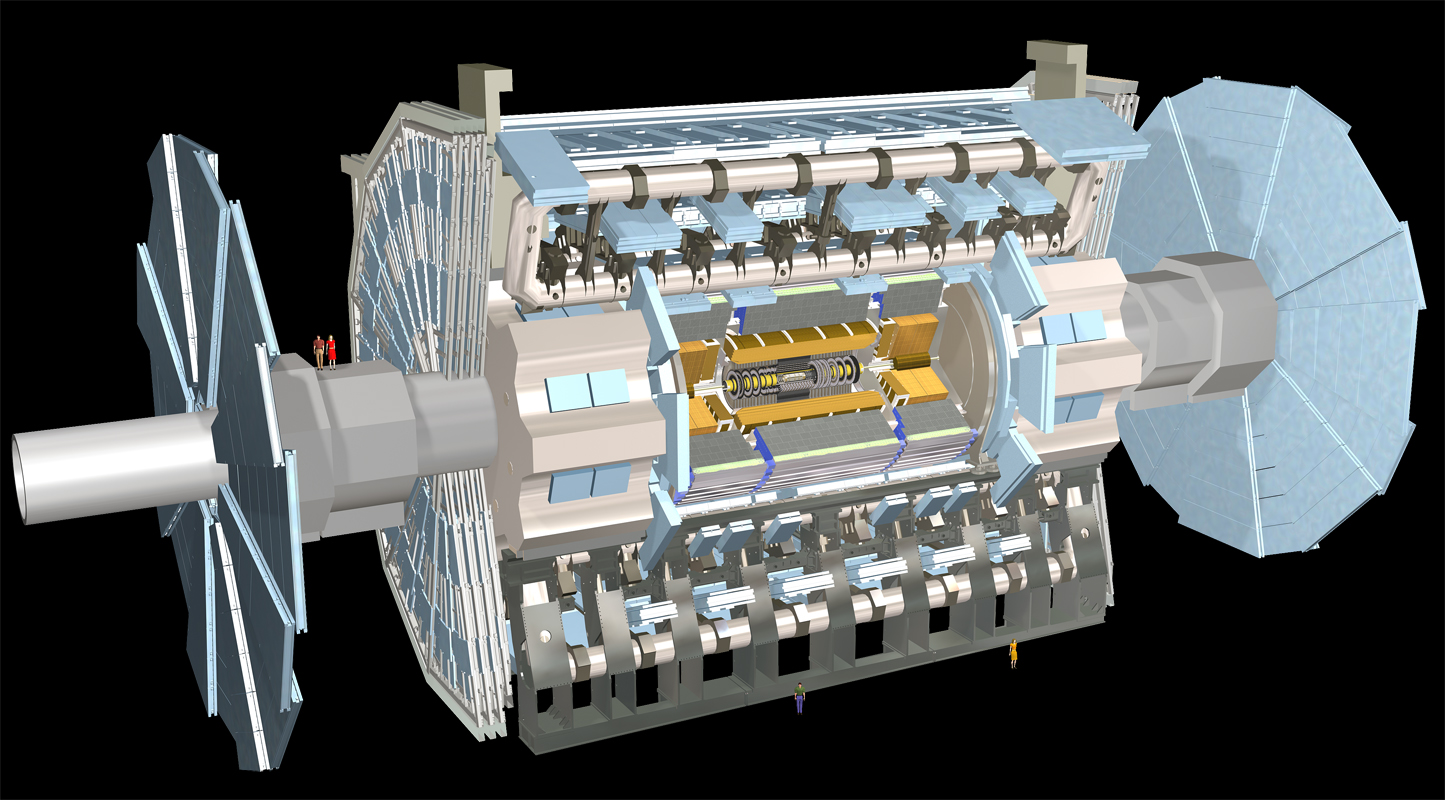
\includegraphics[scale=0.6]{ATLAS.jpg}
\caption{Rappresentazione dell'esperimento ATLAS.}
\label{fig:ATLAS}
\end{figure}

\noindent ATLAS \`e un rivelatore cilindrico di 25 m di diametro e 46 m di lunghezza, dal peso di 7000 tonnellate. Il suo campo magnetico \`e prodotto all'interno da un solenoide, all'esterno da un grande magnete toroidale (si veda la figura \ref{fig:ATLAS}), capace di raggiungere i 2 T nel punto di interazione.\\
Anche CMS \`e un cilindro, ma il suo campo magnetico di 3.8 T \`e interamente prodotto da un grande solenoide centrale, le cui linee di campo sono chiuse da una rilevante quantit\`a di ferro, che serve anche da assorbitore per le particelle che lo attraversano.\\
Entrambi gli esperimenti sono strutturati in tre strati principali che avvolgono completamente la linea di fascio attorno al punto di interazione. A ridosso dell'anello di accelerazione si trovano gli array di rivelatori al silicio, necessari per precise misure posizionali delle tracce cariche. Nel secondo strato, si trovano gli apparati calorimetrici: all'interno il calorimetro elettromagnetico, per la misura dell'energia e posizione di elettroni e fotoni, all'esterno il calorimetro adronico. La struttura pi\`u periferica serve per l'identificazione dei muoni. Gli intensi campi magnetici permettono di misurare il momento e la carica delle particelle elettricamente cariche, che vengono deflesse per effetto della forza di Lorentz.\\
Viste le analogie strutturali e gli scopi comuni tra i due, elenco di seguito le differenze:
\begin{itemize}
\item {\itshape Tracciatori:} hanno una struttura sostanzialmente identica e presentano solo una differenza nella risoluzione del momento trasverso $p_T$, migliore in CMS (principalmente a causa del campo magnetico pi\`u intenso): $\sigma_{p_T}/p_T \approx 5 \cdot 10^{-4} p_T + 0.01$ per ATLAS; $\sigma_{p_T}/p_T \approx 1.5 \cdot 10^{-4} p_T + 0.005$ per CMS.
\item {\itshape Calorimetri elettromagnetici:} a CMS il calorimetro elettromagnetico \`e interamente contenuto all'interno del solenoide, mentre in ATLAS \`e situato al suo esterno. Ci\`o comporta una perdita di energia delle particelle ed un conseguente peggioramento nella risoluzione. Il calorimetro a cristalli di tungstenato di piombo di CMS ha una risoluzione sull'energia $\sigma_E /E \approx 3\%/\sqrt{E}$; quello a sandwich di argon liquido pi\`u assorbitori di piombo di ATLAS ha risoluzione $\sigma_E / E \approx 10\%/\sqrt{E}$.
\item {\itshape Calorimetri adronici:} nel caso di CMS, soltanto una parte del calorimetro adronico \`e inclusa nel solenoide, ed essa non basta per assorbire completamente le particelle adroniche; si \`e perci\`o provveduto ad aggiungere un ulteriore strato calorimetrico al di fuori del magnete. Questa segmentazione abbassa il potere risolutivo. Il calorimetro a sandwich di ferro e scintillatore/rame ed argon liquido di ATLAS ha una risoluzione $\sigma_E /E \approx 50\%/\sqrt{E} + 0.03$ GeV; quello a ottone e scintillatore di CMS $\sigma_E /E \approx 100\%/\sqrt{E} + 0.05$ GeV.
\item {\itshape Spettrometri per identificare i muoni:} in entrambi gli esperimenti, i rivelatori di muoni posti all'esterno del calorimetro, possono ricostruire la traccia del muone in maniera a s\'e stante (``standalone''). La particolare geometria per il sistema di magneti in ATLAS permette delle risoluzioni nettamente migliori nel momento in configurazione standalone, che resta attorno al 10\% anche ad energie prossime ad 1 TeV. CMS invece risulta pi\`u preciso combinando le informazioni delle camere per i muoni con quelle dei tracciatori (7\% ad 1 TeV rispetto al 35\% per gli standalone).
\end{itemize}
\subsection{Altri esperimenti}
Per completezza, riassumo in breve gli scopi degli altri due esperimenti di LHC.
\begin{itemize}
\item ALICE (A Large Ion Collider Experiment) si occupa principalmente di studiare le collisioni tra nuclei pesanti (piombo) alle energie elevate disponibili ad LHC, con l'obiettivo di esplorare meglio la fisica adronica ad elevate densit\`a, in condizioni in cui si forma una nuova fase detta quark-gluon plasma, di fondamentale interesse per comprendere a fondo la QCD.
\item LHCb (Large Hadron Collider beauty) \`e un rivelatore per lo studio del quark b, in particolare per le violazioni di CP e per fenomeni rari associati agli adroni che lo contengono. L'obiettivo di queste ricerche \`e cercare una risposta per il problema dell'asimmetria materia-antimateria.
\end{itemize}
\clearpage
